\section{Fazit und unser Score}
Für die Analyse des kompletten Datensatzes verwendeten wir die BDT-Methode mit dem Parametersatz, der die besten Trainingswerte erreichte. (siehe Abschnitt \ref{sec:bdt_optimization}) Die Eingabevariablen wurden nicht transformiert und der volle Variablensatz wurde verwendet. Der erreichte AMS-Wert liegt bei
\begin{equation}
2.54
\end{equation}

\begin{figure}[htp]
\begin{center}
  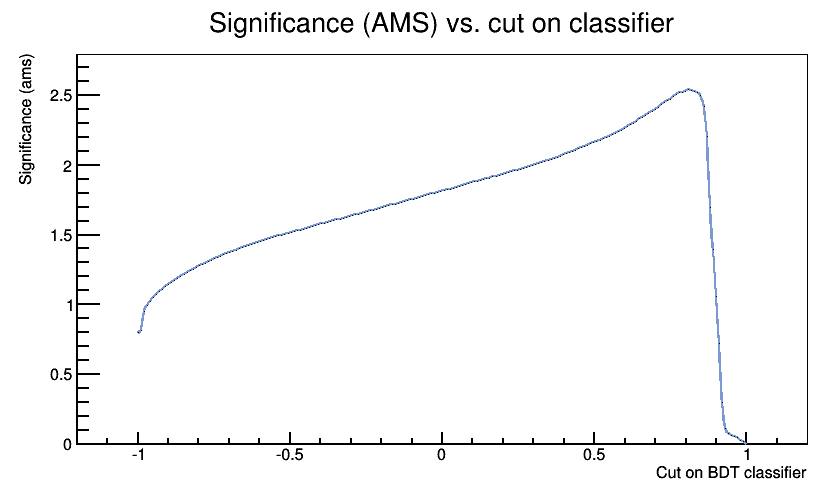
\includegraphics[width=0.7\linewidth]{sections/conclusion/AMS_vs_Cut_cropped.png}
 \caption[]{}
\label{fig:bdt_Shrinkage}
\end{center}
\end{figure}